This chapter will explain in detail how the Flink Backtracking tool written along side this thesis works and how it is used. It is composed of two parts, the frontend part that shows the results in the IDE and the backend part that has to be included in the project that sends the information to the frontend. This chapter is thus split into multiple paths:
\begin{enumerate}
  \item[\ref{fbManual}] User manual
  \item[\ref{fbBackend}] Backend architecture
  \item[\ref{fbFrontend}] Frontend architecture
  \item[\ref{fbState}] State of the program
\end{enumerate}

\section{User manual}
\label{fbManual}

\paragraph{Introduction to the Flink Backtracking Tool}
The Flink Backtracking Tool allows the user to see what data was read at each data stream and what data lead to the result at the next data stream. The Flink Watchpoint mechanism is used which injects a barrier with an indentifier every so often. The data between each of these barriers at each data stream is thus the result of the data between the same barriers plus the transformation of the previous data stream. Thus the exact result of each data stream can be seen which is not possible with step by step debugging.

\paragraph{Prerequirements} There are a few prerequirements that have to be met to make the progrgam work appropriatly. First and foremost it has to be a Flink application as it can only track Flink data streams. Also because it is using the watchpoint mechanism of Flink all requiremts that go along with that have to be met. This means each datastream has to support rolling back data in cases of a failure. Because of this requirement it is currently only possible to use data that comes from some sort of big data storage. In the following examples Apache Kafka will be used.

Using the program is an easy process. The "FlinkBacktracking.jar" has to be integrated into the Flink application that is being developed and the "FlinkBacktrackingIntelliJPlugin.jar" has to be activated in IntelliJ to see the results of the Tool. There is only one line needed to enable the tool itself, although checkpointing still has to be enabled manually:

\begin{lstlisting}[caption={How to use the Backtracker}]
env.setStreamTimeCharacteristic(TimeCharacteristic.EventTime);
env.enableCheckpointing(1000);
FlinkBacktrack backtracker = new FlinkBacktrack(env);
\end{lstlisting}

Where "env" is the Execution Environment. Any number of watchpoint behavior is possible, in this example it is set to inject a berrier after the specified amount of time. Once the Backtracker is initilised it can be used by adding each datastream that the developer wants to be watched to the tool. This is done in the following way:

\begin{lstlisting}
backtracker.track(dataStream, "Transition name");
\end{lstlisting}

Where "dataStream" is the dataStream that should be tracked and "Transition name" is an arbitrary name that is used to show the results under. This step has to be repeated for each data stream that should be watched. Once these steps are done the developer can open the "Flink Backtracking View" by clicking on the button with the same name on the lower right side of IntelliJ and start the application.

\subsection{Debugging a Program with the Backtracker}
Once the plugin has been configured the application can be started. Each piece of data that is being processed by the application will show up in the "Flink Backtracker" tab in IntelliJ as well. The first tabs that are shown are the different data streams. Each watched data stream has its own tab. Each of these tabs contains a list of watch points that passed since the program was started and each of these includes the data that was processed by that data stream at the time of the watchpoint.

\begin{figure}[h!]
    \centering
      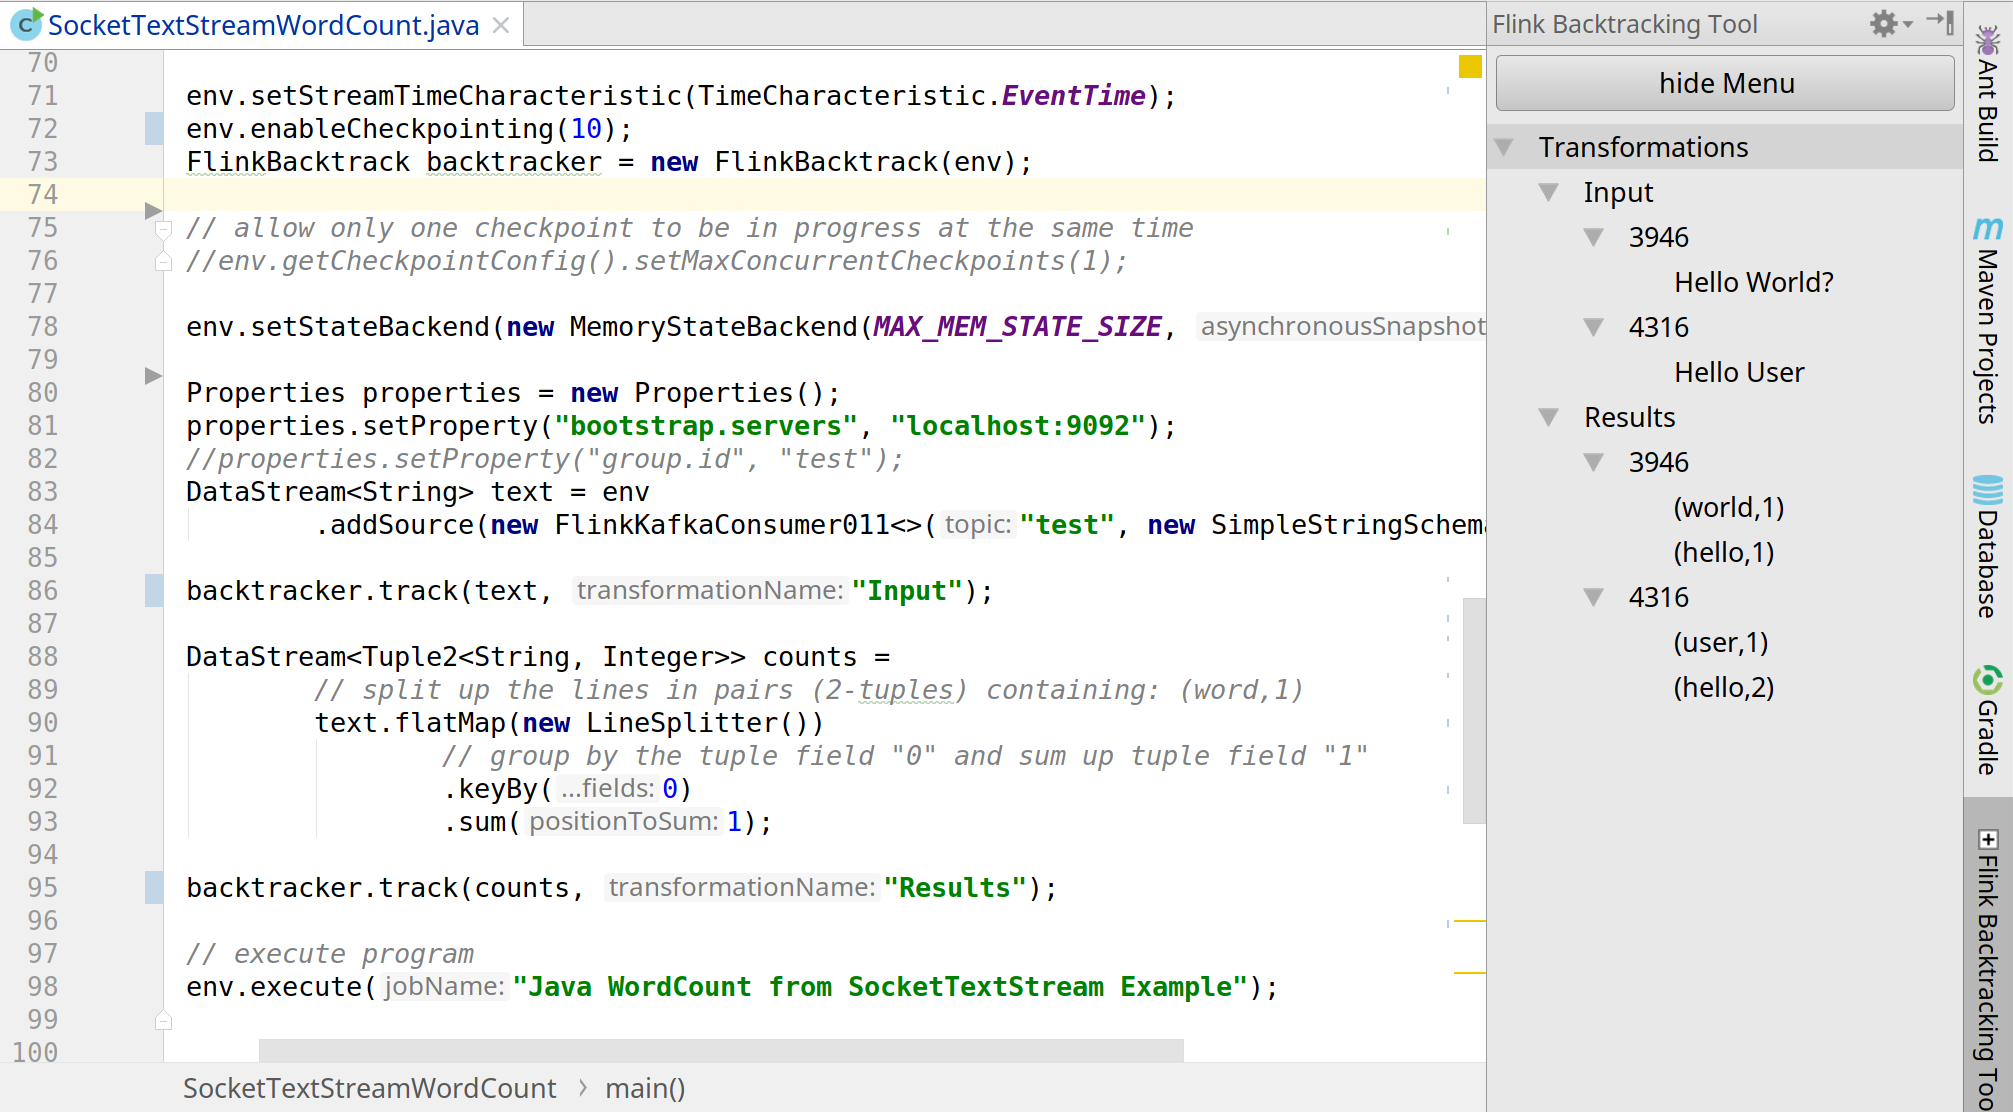
\includegraphics[width=0.9\textwidth]{FlinkBacktrackerIntelliJPluginExample.png}
      \caption{Backtracking Example}
      \label{flinkBacktrackingExample}
\end{figure}

\paragraph{} The example \ref{flinkBacktrackingExample} shows a good use-case for the tool. The developer can easily see that the input of the program was successfully received by the first data stream. He can also see that the application is removing special characters and converting all capital letters. Because the content of the second data stream (result) is not only depending on the data stream that came before (input) but also on all the data that was processed by the stream previously. Thus the "hello,2" in the result transition at watchpoint 4316.

\section{Backend architecture}
\label{fbBackend}
The Backend is composed of two parts one is the function that is collecting the data and sending it to the frontend the other is main class that is used to set up the function in the correct way to ensure that the function can gather all the neccesary information.

\paragraph{} The following example (\ref{dataFlowNoBacktracker}) helps to underline how the Flink application is set up so that the data can be sent to the frontend.

\begin{figure}[h!]
    \centering
      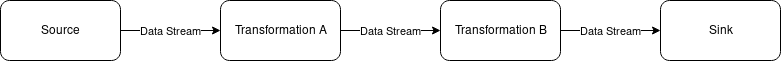
\includegraphics[width=0.9\textwidth]{DataFlowNoBacktracker.png}
      \caption{Dataflow without the Backtracker}}
      \label{dataFlowNoBacktracker}
\end{figure}

\ref{dataFlowNoBacktracker} is a simple application with 2 transformations much like the Word Count application used throughout this thesis. The first transition is reading the input and the second is modifying it. At each transition we split the data stream and send an exact copy to another transformation that is part of the Backtracker that sends it to the front end. That means that with the Backtracker enabled the earlier diagramm now looks like this: \ref{dataFlowWithBacktracker}

\begin{figure}[h!]
    \centering
      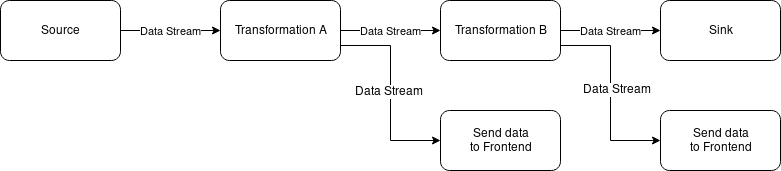
\includegraphics[width=0.9\textwidth]{DataFlowWithBacktracker.png}
      \caption{Dataflow with the Backtracker enabled}
      \label{dataFlowWithBacktracker}
\end{figure}

This ensures that the data is sent to the frontend but fails to show which pieces of information are related to each other. Because of that it is necessary to add watchpoints to the system. The way that Flink handles watchpoints is simple: They are injected at the beginning of the application as part of the data stream, and each time a transformation receives one it injects the same one back at its output at the same position. Each watchpoint is identified by a unique number and is used as a grouping method in this tool. Flink does not allow the current checkpoint to be read out because there can be multiple active at the same time in different parts of the application. The only way to get the current checkpoint for a given transition is by saving the last checkpoint that was read by the transition. The snapshotState method is called by the Task Manager each time a new watchpoint is registered. The following line then saves the checkpointId as a field of the class so that the most recent watermark is always available:

\begin{lstlisting}[caption={Save Watermark}]
@Override
public void snapshotState(FunctionSnapshotContext context)
throws Exception {
  currentWatermark = context.getCheckpointId();
}
\end{lstlisting}

When sending messages to the frontend the current watchpoint can then be added.

\paragraph{Sending Data}

Another important step along the way is sending the data to the frontend. This is done by astablishing a socket connection to the frontend (the frontend is the server) and sending Java objects over it.

\section{Frontend architecture}
\label{fbFrontend}
The frontend architecture is pretty straigt forward. A view is created and populated with a tree view together with a socket server that is avaiting messages from clients. Once it recieves a message it checks if the transformation and/or watchpoint is already present in the tree and fills the data to the correct location. The server can never stop intelliJ from working as it is running in a seperate thread, thus ensuring that any problems with the connection are isolated.


\section{State of the program}
\label{fbState}
The backtracker tool is in a working state, that being said it is not tested in the most vigorues way possible and there are still a few features that would really enhance the usability like being able to save the results.

\paragraph{Saving results}
At the moment the only way the data can be displayed is by using the IntelliJ plugin. Because the messages are sent by the internal transformation a second transformation could be written that instead of sending the data to the IntelliJ plugin saves it in a data base or logs it to a file. When creating the Backtracker a second constructor was needed to specify which Backend function to use.

\paragraph{Better UI}
The UI still lacks a few features that would drasticly increase the ease of the program like clearing old results or saving the tree directly from there.
